\section{Format string bug}

This vulnerability allow to perform arbitrary memoryreads and even arbitrary
memory writes. This is extremly powerfull in order to for example defeat
stack canaries, e.g., by reading the canary from memory, or by overwriting the
global canary, or overwriting a return address without touching the canary.


\url{https://axcheron.github.io/exploit-101-format-strings/}

\url{https://codearcana.com/posts/2013/05/02/introduction-to-format-string-exploits.html}

\subsection{Introduction}
\subsubsection{variadic functions}
In C {\bf variadic functions} are declared by ending the list of their arguments with
\verb+...+ . For example, printf() can be declared as:
\begin{verbatim}
int printf(const char *fmt, ...);
\end{verbatim}

The C compiler handles variadic functions by {\bf not checking} the number and
types of the arguments that are passed to the function in the “ \verb+...+”
position. Any arguments found in the call site are put in their place in the
registers or on the stack. When the callee function needs one of these
arguments, it will read the expected location for that argumenti (register or
stack). The function has no way to know if the argument was actually passed by
the caller, or if the argument type was the correct one: it will read whatever
the expected argument location currently contains, interpreting it as a value
of the expected type. Correct functionality entirely depends on conventions
between the caller and the callee.

\subsubsection{Format string}
{\bf Format strings} are the control strings that are passed to the
\verb+printf()+ family of functions and contain the output template for the
functions. These functions are vulnerable whenever the attacker can control the
format string itself.

In the \verb+printf()+ family of functions, the convention is that each format
specifier will take an additional argument.

In 32b systems, the first argument is on the stack, just below the pointer to
the format string; the second argument is below the first one, and so on. In
64b systems the first 6 arguments (including the pointer to the format string)
are passed in registers and all additional arguments are pushed on the stack.

Consider a statement like this:
\begin{verbatim}
printf(buf);
\end{verbatim}
where the contents of \verb+buffer+ are controlled, even in part, by the attacker.
The programmer simply wanted to print a string, but \verb+printf()+ will
interpret any \verb+%+ character inside buf as a {\bf format specifier}. Each
one of these format specifiers needs a corresponding argument and
\verb+printf()+ will read the registers or the memory locations where that
argument should have been, under the control of the attacker.

{\bf Interesting format specifier}:
\begin{itemize}
    \item \verb+%p+: pointer
    \item \verb+%x$p+: pointer + offsert (\verb+x+)
    \item \verb+%s+: string
    \item \verb+%ms+: string of at least \verb+m+ bytes    
    \item \verb+%.ms+: string of at most \verb+m+ bytes    
    \item \verb+%m.ms+: string of exactly \verb+m+ bytes    
    \item \verb+%d+: int
    \item \verb+%c+: char (1 byte)
    \item \verb+%x+: hex (4 bytes)
    \item \verb+%lx+: long hex (8 bytes)
\end{itemize}
i
\subsubsection{printf as a machine}

{\bf Probably the best way to reason about what we can do, is to consider
\verb+printf()+ as anew machine with its own programming language}.  The format
string is the program and the instructions are normal characters and format
specifiers. The \verb+printf()+ machine has its own instruction pointer, pointing
to the next character/format specifier to “execute”. This pointer only moves
forward without jumps in either direction: there are no loops and no conditional
branches.

The instructions update the machine state which, besides the instruction
pointer, contains the following:
\begin{itemize}
    \item an argument pointer, pointing to the argument to be used by the
            next format specifier;
    \item an output counter, containing the number of characters that have been
        output so far.
\end{itemize}

The machine also produces output.

surprisingly the machine can also write into memory. The \verb+%n+ specifier’s
argument must be a pointer to an integer variable. \verb+printf()+ will execute
it by writing the current output counter into the variable.

\subsection{Stack leaking}

In 32b systems, a sequence of \verb+%x+ specifiers will cause \verb+printf()+
to print successive lines from the stack. In 64b systems, the first 5
\verb+%lx+ will print the contents of the \verb+rsi+, \verb+rdx+, \verb+rcx+,
\verb+r8+ and \verb+r9+, and any additional \verb+%lx+ will start printing
successive stack lines.

The only real difficulty comes from space limitations in the
controlled buffer, since the argument pointer is only moved forward by a format
specifier. Any format specifier will move the argument pointer by at least one
stack line (which is 4 bytes in 32b and 8 bytes in 64b systems), since arguments
are always aligned to stack-lines. Assume that the buffer size is \verb+s+, the attacker
can only move the argument pointer by \verb+s/2+ lines, which may not be enough
to reach the desired information on the stack.

\subsection{Random access to arguments}

The format string can also access its arguments in
random order using the \verb+%n$+ syntax, which selects the \verb+n+th argument
directly.

This syntax can be used to easily overcame the space limitations of the
buffer. If we know that the desired information is \verb+n+ stack-lines
below the pointer to the format string, \verb+%n$x+ will print it directly on 32b
systems, while \verb-%(n + 5)$lx- will do the same on 64b ones.

This was possibile in old versions of glibc, or even in modern ones if some
complile options have not been enabled (\verb+FORTIFY_SOURCE+). According to
the standard:
\begin{itemize}
    \item random access and sequential argument access are mutually exclusive
    (the same format string cannot contain both forms) 
    \item once all the argument numbers have been collected, there cannot be
        any gaps remaining.
\end{itemize}

If the no-gaps rule is enforced, random access arguments cannot be used to
overcome the space limitations in the buffer. When glibc allows this behaviour,
though, it simply assumes that all non-referenced argu ments occupy one
stack-line each.

There may be limitations, however, on the maximum argument number, so you
cannot usually use this feature to read memory that is very far on the stack
or, most importantly, at addresses lower than the stack top.

\subsection{Arbitrary Reads}

Arbitrary memory read can be achieved when the format string itself is stored
on the stack and can be reacherd by the argument pointer like in the following
example
\begin{verbatim}
int funn(void) {
    char buffer[30];
    ...
    gets(buffer);
    printf(buffer);
    ...
}
\end{verbatim}

 \begin{figure}
  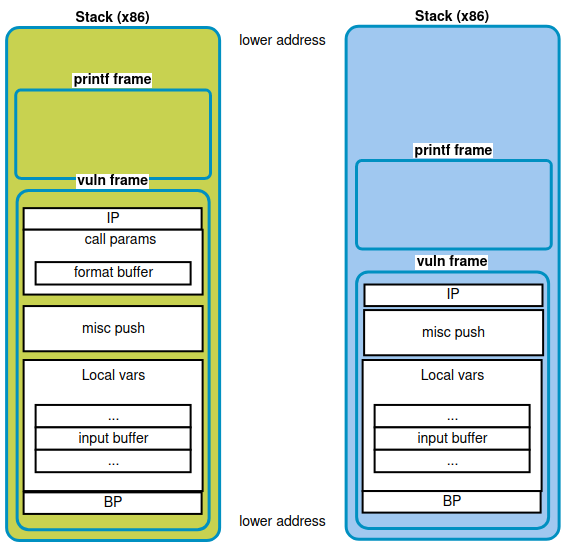
\includegraphics[width=\linewidth]{binary/exploit_linux/images/format_string_stack.png}
  \caption{Anatomy of the stack before calling printf}
  \label{fig:format_string_stack}
\end{figure}

Assume that the format string (or a copy)is stored at {\bf offset \verb+o+}
(i.e. is store at \verb+o+ stack-lines below
the pointer passed to \verb+printf()+). Then, the \verb+o+th argument on 32b
systems, (\verb-o+5-th argument in 64b) , will take its value from
the beginning of the format string itself. The attacker, therefore, can put
both the instructions and their arguments in the same format string “program”.

Considering the \verb+%s+ instruction which normallyprints a string, when reinterpreted as in
instruction for the \verb+printf()+ machine, it prints the contents of memory
starting from the address specified by its argument and stopping at the first
\verb+null+ byte. If the attacker can choose the address that the instruction will use, this
is an arbitrary-memory-read instruction.

For example, in a 32b binary, in order to read from address \verb+0x11223344+
considering that the format string is stored offset 3 the following buffer must
be provided:
\begin{verbatim}
\verb+\x44\x33\x22\x11%c%c%s+. 
\end{verbatim}

Note that the buffer must be stack-line aligned, which may not always be the
case. This is achieved by inserting some padding bytes at the beginning before
writing the address.
\begin{verbatim}
\verb+,,\x44\x33\x22\x11%c%c%s+. 
\end{verbatim}


\subsubsection{non-null bytes target}
A problem may arise if there are no null bytes to stop \verb+printf()+ before it
reaches some non-readable memory that may cause the process to be terminated.
This can be solved  by using a \verb+%.ms+ instruction, that will
always read (and print) at most \verb+m+ bytes.

\subsubsection{null bytes address}
\verb+Null+ bytes in the address may be a problem, since the \verb+null+ byte
is an halt instruction for \verb+printf()+. 

In the format string above, for example, a \verb+null+ byte in the address
would stop the \verb+printf()+ before it could even see the first \verb+%x+
instruction. However, if null bytes in the format string are otherwise allowed,
this is not really a problem: the address can be put after the instructions.

taking back the previous example, in order to read address \verb+0x44002211+,
the buffer should be:
\begin{verbatim}
%c%c%c%s\x11\x22\x00\x44
\end{verbatim} 

Note that the string containsan additional \verb+%c+ to move the argument
pointer one step more. 

With random access is availabe the buffer would be
\begin{verbatim}
%4$sAAAA\x11\x22\x00\x44
\end{verbatim}. 

If \verb+null+ bytes are not allowed anywhere, but the address only contains null bytes
in the most significant positions, the attacker may still succeed by putting the
non-null bytes of the address at the very end of the string and exploiting any
\verb+null+ bytes that may already follow the string by chance.


\subsection{Arbitrary Write}

\verb+%n+ take a pointer and wrties there {\emph the number of characters
written so far}.

ontrolling the output counter is less difficult than it may seem, since an
instruction like \verb+%mc+ will always increment the output counter by exactly
\verb+m+.  If there are also other instructions in the format string, you must
be careful to control the number of bytes that they output. This can be
accomplished by adding width specifiers to each one of them, but be aware of
the exact semantics: \verb+%ms+ will always output at least \verb+m+ bytes,
while \verb+%.ms+ will always output at most \verb+m+ bytes. If you want
exactly \verb+m+ bytes, you need both: \verb+%m.ms+.a


Another possible difficulty comes from the fact that, if you want to write a
very large value (say, the address of a function), you may have to output an
impractical or impossibly large number of bytes. 

This difficulty of writting very large value can be overcome by using the
\verb+%hn+ instruction, that truncates the counter to a short (2 bytes), or
even \verb+%hhn+, that truncates it to a char. Using the latter instruction 4
times at consecutive addresses, for example, you can write any 32 bit value one
byte at at time, always incrementing the output counter by at most 255 bytes.

Note that, if the LSB of the counter is \verb+c+ and you need a value 
\verb+v < c+, you cannot subtract from the counter, but you can increment it by
\verb|256 - c + v| bytes and the LSB will become \verb+v+

For example, the following buffer will write the value \verb+0x44552233+
assuming the LSB of the output counter is initially 32.
\begin{verbatim}
%36c%hhn%17c%hhn%205c%hhn%17c%hhn
\end{verbatim}

\begin{itemize}
    \item \verb-32+36 = 68 = (44)16-
    \item \verb-68 + 17 = 85 = (55)16-
    \item \verb-205 + 85 = 290 = (122)16-
    \item \verb-290 + 17 = 307 = (133)16-
\end{itemize}

so to write this value to a memory address \verb+0x01020304+ considering that
the format string is stored at offset 0, the following buffer must be provided:
\begin{verbatim}
AAAA\x04\x03\x02\x01BBBB\x05\x03\x02\x01
CCCC\x06\x03\x02\x01DDDD\x07\x03\x02\x01
%36c%hhn%17c%hhn%205c%hhn%17c%hhn
\end{verbatim}

The \verb+AAAA+, \verb+BBBB+, and so on, serve as dummy arguments for the c
instructions and to re-align the next argument to the stack-line. The other
arguments are the addresses of all the bytes of the target memory location,
starting from the least significant one.

the 32 value for the initial counter previously stated comme from the size of
the prepending string containing the address.


\subsection{pwntools}

fmStr object from pwntools allow to easily exploit this bug. Usefull mostly to
find the offset on the stack and to perform arbitrary write.


